\chapter{Описание используемых методов} \label{ch2}
	
% не рекомендуется использовать отдельную section <<введение>> после лета 2020 года
%\section{Введение} \label{ch2:intro}


\section{Методы обработки изображений реализованные в пакете ProStack} \label{ch2:title-abbr} %название по-русски
В данной работе производится модификация и улучшение методов обработки изображений реализованных в пакете ProStack.\cite{Mastersthesis}

В пакете ProStack реализованы стандартные и проблемно-ориентированные методы
обработки изображений а также методы для получения количественных данных из изображений, полученных на световом или конфокальном микроскопе. Пакет имеет графический
интерфейс, для построения сложных сценариев. \cite{Article}

Механизм обработки изображения в данном пакете представляет из себя
своего рода конвеер - множество зависимых
друг от друга различных операций, записанных в один сценарий.

Все методы в рамках пакета разделены на десять классов.\cite{Article}
\begin{itemize}
	\item Комбинирование (Получение одного изображения из нескольких входов)
	\item Выделение объектов
	\item Корректировка (Повышение качества изображения)
	\item Сегментация (Разделение изображения на части/зоны)
	\item Восстановление
	\item Морфология (Морфологические операции)
	\item Геометрия (Изменение свойст изображений)
	\item Преобразование
	\item Арифметика (Алгебраические операции)
	\item Разное
\end{itemize}


\begin{figure}[H]
	\centering
	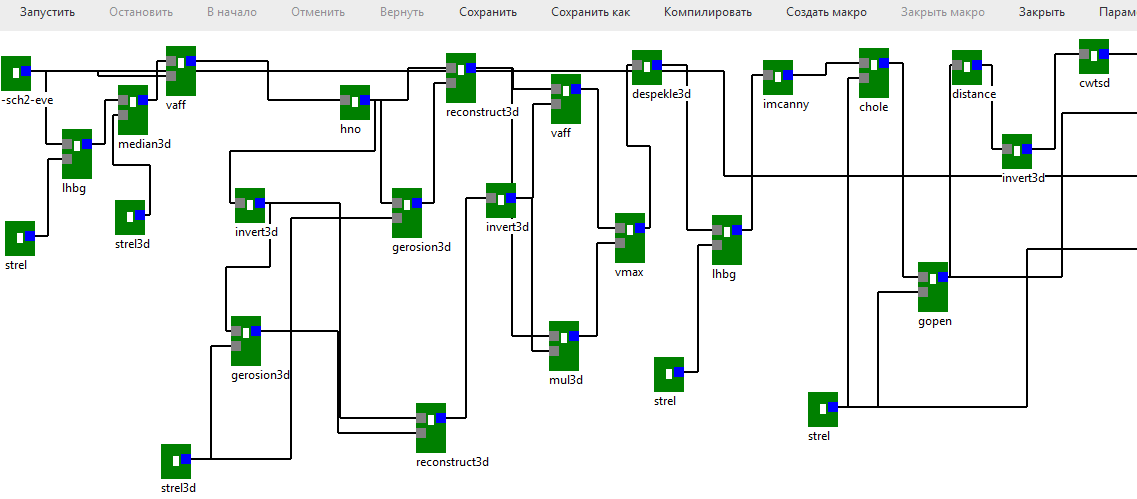
\includegraphics[width=13cm, height=5cm]{blocks}
	\caption{Графический сценарий обработки трехмерного изображения из пакета ProStack}
	\label{descr}
\end{figure}

Рассмотрим некоторые морфологические операции, которые реализованы в пакете, а также применялись для извлечение количественных данных из изображений мозга мушки.

Для улучшения сегментации(например обработки фона) применяют операцию морфологического размыкания - комбинацию операций эрозии и наращивания. Расссмотрим операции на простом примере. Допустим мы имеем следующее  изображение и структурный элемент: \cite{Incollection}
\begin{figure}[H]
	\minipage{0.48\textwidth}
	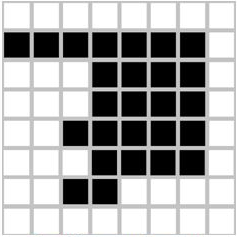
\includegraphics[width=5cm, height=5cm]{morf_bin_example}
	\caption{Изображение I}\label{morf_bin_example}
	\endminipage\hfill
	\minipage{0.48\textwidth}
	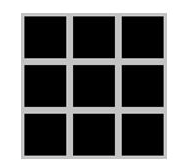
\includegraphics[width=5cm, height=5cm]{morf_struct_example}
	\caption{Структурный элемент S}\label{morf_struct_example}
	\endminipage\hfill
\end{figure}

	\textbf{Наращивание} — Структурный элемент "пробегает" по всем пикселам бинарного изображения. Если  начало координат структурного элемента совпадает с пикселем изображения, то производится логическое сложение структурного элемента с пикселями изображения. Результат  записывается в выходное изображение. \cite{Incollection}
	
	\begin{figure}[H]
		\centering
		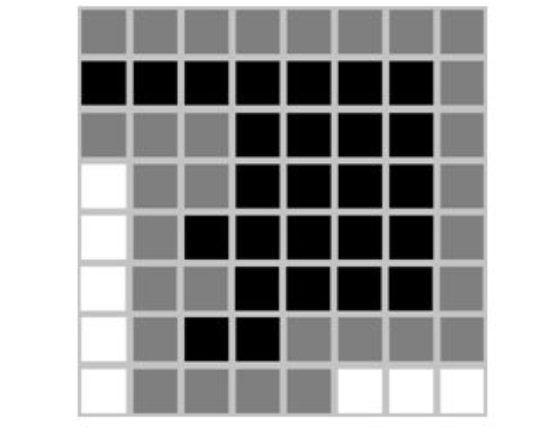
\includegraphics[width=5cm, height=5cm]{morf_narach}
		\caption{Наращивание изображения I структурным элемнтом S}
		\label{morf_narach}
	\end{figure}
	
	\textbf{Эрозия} — Структурный элемент также "пробегает" по всем пикселам изображения. При этом, если каждый пиксель структурного элемента совпадет с пикселями изображения - происходит логическое сложение пикселя находящегося по центру структурного элемента с пикселем изображения. Результат логического сложения также записывается в выходное  изображение. \cite{Incollection}
	
	\begin{figure}[H]
		\centering
		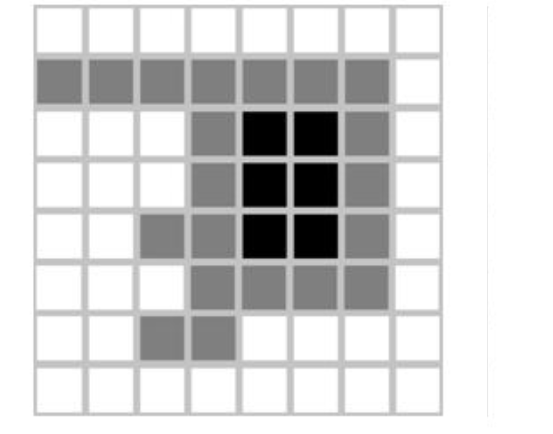
\includegraphics[width=5cm, height=5cm]{morf_eroz}
		\caption{Эрозия бинарного изображения I структурным элемнтом S}
		\label{morf_eroz}
	\end{figure}
	
	\textbf{Размыкание} — эрозия хороша тем что позволяет избавляться от малых объектов представляющих из себя шум. Также из-за этой операции размеры объектов уменьшаются.Это часто неприемлимо для задачи, поэтому после эрозии применяют операцию наращивания используя тот же структурный элемент.\cite{Manual}
	\begin{figure}[H]
		\centering
		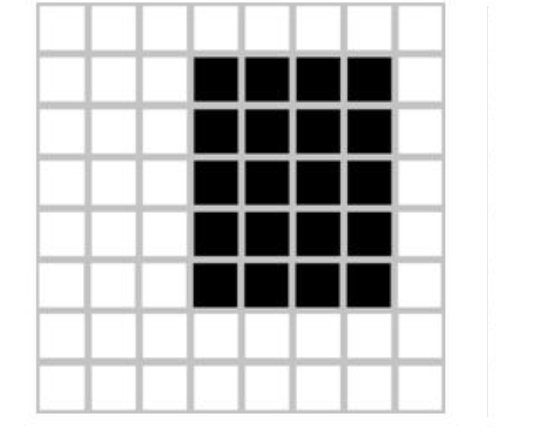
\includegraphics[width=5cm, height=5cm]{morf_razmik}
		\caption{Размыкание бинарного изображения I структурным элементом S}
		\label{morf_razmik}
	\end{figure}

Можно сделать в другом порядке - получится операция \textbf{Замыкания}. В таком случае наращивая изображение можно "заполнить" щели. Но чтобы избежать увеличение изображения - производится последующее применение операции эрозии. \cite{Manual}




Далеее рассмотрим довольно распространенную операцию в обработе изображений - \textbf{выделение границ}. Данная операция, а именно оператор Кэнни был применен в этой работе для выделения комплексов молекул РНК.

Границей называется изменение яркости на изображении. Она проходит между двумя отличающимися по интенсивности областями. Выделение границ позволяет получить количественные данные из изображений о количестве, площади, размерах областей/зон. Для обнаружения границ могут быть использованы маски.\cite{Misc}


Рассмотрим операторы \textit{Робертса, Собеля, Превитта} и алгоритм \textit{Кэнни}.

\begin{center}
	\textit{Фильтрация}
\end{center}
 Дадим определение \textbf{разрывности} - резкое изменение значений интенсивности. Довольно общим методом поиска разрывности является использование скользящей маски, представляющей из себя обычно квадратную матрицу (или матрица коэффициентов).Применение маски к изображению называют фильтрацией.\cite{Phdthesis}
	Схема  применения маски показана на рисунке \ref{mask}:
	\begin{figure}[H]
		\centering
		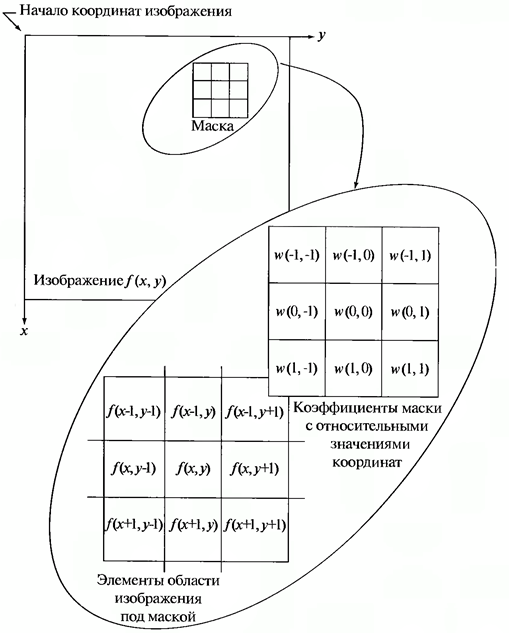
\includegraphics[width=14cm, height=12cm]{mask}
		\caption{Фильтрация изображения маской коэффициентов}
		\label{mask}
\end{figure}

Применение маски основано на скольжении маски вдоль изображения по вертикали и горизонтали и вычислении некоторой величины R - сумма произведения значений каждого пикселя в области, покрытой в некоторый момент маской на соотвествующие значения коэффициентов маски.\cite{Phdthesis}
Для примера на рисунке \ref{mask}, значение \textbf{R}  в точке \textbf{(x,y)} вычисляется как:
$R = w(-1, -1) * f(x - 1, y - 1) + w(-1, 0) * f(x - 1, y) + ...w(0,0) * f(x, y) + ... + w(1, 0) * f(x + 1, y) + w(1,1) * f(x + 1, y + 1)$ 

Для определения разрывов используют аналоги производных и градиента.
Производная первого порядка  функции f(x) определяется так:  $\frac{df}{dx} = f(x + 1) - f(x)$.
Вторая :
$\frac{df^2}{dx^2} = f(x + 1) - f(x - 1) - 2f(x)$.\\
Градиент f(x,y) в точке (x,y):\\
$\nabla f = [\frac{G_x}{G_y}] = \dfrac{\frac{df}{dx}}{\frac{df}{dy}}$.\\

Для поиска границ объектов вычисляется модуль градиента $ |\nabla f| $, который равен\\
$|\nabla f| = \sqrt{G_x^2 + G_y^2}$.
{\begin{center}
		Оператор Робертса
\end{center}}
Предположим, что матрица размером 3х3, показанная на рисунке \ref{Robert_1} представляет пример участка изображения, элементы являются значениями интенсивности.\cite{Phdthesis}


\begin{figure}[H]
	\centering
	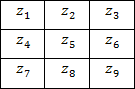
\includegraphics[width=5cm, height=3cm]{Robert_1}
	\caption{Окрестность 3х3}
	\label{Robert_1}
\end{figure}  

Определение частных производных первого порядка для оператора Робертса:  $G_x = z_9 - z_5$ и $G_y = z_8 - z_6$
Таким образом можно обработать всё изображение с помощью оператора Робертса
описываемого матрицами на рисунке \ref{Robert_2} и воспользоваться процедурой фильтрации.\cite{Phdthesis}

\begin{figure}[H]
	\centering
	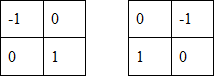
\includegraphics[width=4cm, height=2cm]{Robert_2}
	\caption{Маски оператора Робертса}
	\label{Robert_2}
\end{figure}

Для масок размеров 2х2 из-за отсуствия центрального элемента ухудшается результат выполнения фильтрации. Данный минус компенсируется высокой скоростью обработки всего изображения.

{\begin{center}
		Оператор Превитта
\end{center}}

Оператор Превитта тоже работает с областью 3х3, но градиенты вычисляются иначе:
$G_x = (z_7 + z_8 + z_9) - (z_1 + z_2 + z_3)$ и $G_y = (z_3 + z_6 + z_9) - (z_1 + z_4 + z_7)$\\
Данные формулы описываются масками на рисунке \ref{Previt_1}.  
\begin{figure}[H]
	\centering
	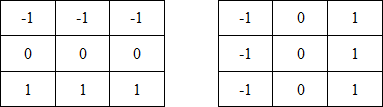
\includegraphics[width=8cm, height=3cm]{Previt_1}
	\caption{Маски оператора Превитта}
	\label{Previt_1}
\end{figure}

{\begin{center}
		Оператор Собеля
\end{center}}
Оператор Собеля в отличие от оператора Превитта использует весовой коэффициент равный двум для средних элементов:
$G_x = (z_7 + 2z_8 + z_9) - (z_1 + 2z_2 + z_3)$ и $G_y = (z_3 + 2z_6 + z_9) - (z_1 + 2z_4 + z_7)$

Данное увеличение коэффициентов направлено на уменьшение эффекта сглаживания.\cite{Phdthesis}
\begin{figure}[H]
	\centering
	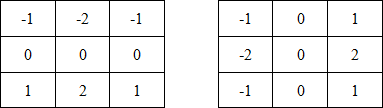
\includegraphics[width=8cm, height=3cm]{Sobol_1}
	\caption{Маски оператора Собеля}
	\label{Sobol_1}
\end{figure}

Далее по полученным значениям $G_x$ и $G_y$ после применения масок вычисляетя вектор градиента.
$|\nabla f| = \sqrt{G_x^2 + G_y^2}$. Решение о перепаде интенсивности, то есть наличии границы применяется после сравнение модуля градиента с некоторым пороговым значением (подбирается эмперически).\cite{Phdthesis}



{\begin{center}
		Детектор границ Канни
\end{center}}
Детектор Кэнни является одним из самых популярных алгоритмов поиска границ. Он был разработан Джоном Ф. Кэнни в 1986 году. Ключевым этапом является подавление шума на контурах, что значительно может повлиять на результат выделения. \cite{Misc}
 
Рассмотрим этапы алгоритма детектора границ Кэнни \cite{Booklet}:  \label{canny_algo}
\begin{enumerate}[1.]
	\item \textit{Размытие изображения}. Так как операция выделения границ чувствительна к шуму в изображении, то необходимо этот шум удалить - с помощью гауссовского фильтра.
	
	\item \textit{Поиск градиента яркости изображения}. Далее, сглаженное на первом этапе изображения фильтруют оператором Собеля. То есть вычисялется первая производная по горизонтали $G_x$ и по вертикали $G_y$. Далее вычисляется вектор градиента и его модуль  $|\nabla f| = \sqrt{G_x^2 + G_y^2}$. Направление градиента перпендикулярная границе и расчитывается как $\tan^{-1} (\frac{G_y}{G_x})$.
	
	\item \textit{Подавление не локальных максимумов}. После получения значения модуля и направления для градиента на 2 этапе выполняется удаление пикселей представляющих собой лишние участки границ. То есть, рассматриваются значения пикселей границы в направлении градиента, и удаляются пиксели, значение интенсивности которых не превышает значения двух соседних в рассматриваемом в заданном направлении. Таким образом данный этап позволяет получить более тонкие края границ изображения.
	
	\item \textit{Пороговые значения для границ}. На данном этапе идет отсечение некоторых границ по пороговому значению. Например, допустим заданы два порога \textit{minTresh} и \textit{maxTresh}, тогда любые границы со значениями интенсивности больше \textit{maxTresh} обязательно будут порогами, а те что ниже \textit{minTresh} - удаляются. Все остальные границы значения интенсивностей которых лежат между этими порогами классифицируются в зависимости от того связаны ли они с границами интенсивности которых превышают \textit{maxTresh} или нет.
	
	На рис. \ref{tresh_canny} проиллюстрирована работа совершаемая на данном этапе. Граница А находится выше \textit{maxTresh} и поэтому считается истинной, граница С находится ниже \textit{maxTresh} но связана с А, которая в свою очередь считается границей, в таком случае С также не отсеивается. Но граница В находится ниже \textit{maxTresh} и не имеет связи как С, в таком случае В удаляется. \cite{Booklet}
	
	\begin{figure}[H]
		\centering
		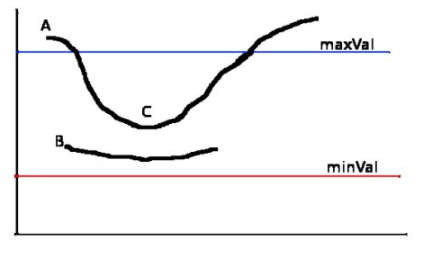
\includegraphics[width=7cm, height=7cm]{tresh_canny}
		\caption{Отсечение найденных границ по пороговому значению}
		\label{tresh_canny}
	\end{figure}
\end{enumerate}


%%%%
%%		
%%  \input{...} commands are used only to sychronize some parts of the text with the author guide. Authors are free to type the text directly in .tex-files   
%%  \input{...} комманды используются только, чтобы синхронизировать части текта с рекомендациями авторам. Авторы  вольны вносить текст непосредственно в файл главы  
%%  


	


	
\section{Инструмент поиска автофлуоресценции. AFid} \label{ch2:sec-abbr} %название по-русски
Данный метод является програмным способом удаления автофлуоресценции \ref{ch1:sec3}. То есть применяется после получения изображения и делает его весьма практичным  так как пользователям не нужно менять свои экспериментальные процедуры.\cite{Conference}	
	
\subsection{Входные данные и требования} \label{ch2:subsec-title-abbr} %название по-русски
Алгоритм принимает на вход два изображения - двухканальное изображение исследуемого объекта, разделенное на два канала. Для разбиения использовался пакет Fiji. \cite{Techreport}
 
Важным требованием алгоритма является то что автофлуоресценция не должна перекрываться реальным сигналом. То есть не должно быть фонового перекрытия между реальным сигналом для конкретного канала и сигналом являющегося автофлуоресцентным.\cite{Conference}

\subsection{Создание маски пересечения}
Маска пересечения двух каналов используется для исключения автофлуресценции. Она содержит только те сигналы, которые присутствуют в обеих каналах, и поэтому содержит интересующие автофлуоресцентные области. Маска строится следующим образом: к каждому из каналов изображение применяется Гауссово размытие с $\sigma = 2$ и с размером Гауссово ядра \textit{k}, расчитываемого по формуле $ k =  2 * ceil(2 * sigma) + 1$, где \textit{ceil} - функция округления вверх. Далее к размытым каналам применяется порог Оцу, которое определяет оптимальное глобальное пороговое значение из гистограммы изображения, и полуются две бинарные маски для каждого канала. Результирующая маска пересечения получается путем применения друг к другу "логического И"     бинарных масок полученных на предыдущем шаге. \cite{Conference}

\begin{algorithm} [H]
\SetKwFunction{algoDTestsFDSCALING}{} 
\SetKwProg{myalg}{Псевдокод алгоритма генерации маски пересечения}{}{} %write in 2nd agrument <<Algorithm>>, <<Procedure>> etc
\nonl\myalg{\algoDTestsFDSCALING}{ 	
	\KwInput{Первый канал - ch1, второй канал - ch2} 	
	\KwOutput{Маска пересечения - result mask}
	sigma = 2\;
	blurred chanel 1=imgaussfilt(ch1) //Гауссово размытие 1 канала\;
    blurred chanel 2=imgaussfilt(ch2) //Гауссово размытие 2 канала\;
	th1 = threshold(blurred chanel 1) //Применение порога Оцу\;
	th2 = threshold(blurred chanel 2)\;
	resmask = th1 \& th2 //логическое И бинарных масок для каждого канала\;
	\Return resmask\;
}
\label{alg:AlgoFDSCALING}
\end{algorithm} 



%Вместо подподпараграфов рекомендовано использовать перечисления.

Перечисления могут быть с нумерационной частью и без неё и использоваться с иерархией и без иерархии. Нумерационная часть при этом формируется следующим способом:

\begin{enumerate}[1.]
	\item в перечислениях {\itshape без иерархии} оформляется арабскими цифрами с точкой (или длинным тире).
	\item В перечислениях {\itshape с иерархией} --- в последовательности сначала прописных латинских букв с точкой, затем арабских цифр с точкой и далее --- строчных латинских букв со скобкой. 
\end{enumerate}


%% Если в дальнейшем нужно сделать сслыку на один из элементов нумеруемого перечисления, то нужно использовать конктрукцию типа:

%\begin{enumerate}[label=\arabic{enumi}.,ref=\arabic{enumi}]
%	\item text 1 \label{item:text1}
%	\item text 2
%\end{enumerate}
%\ref{item:text1}.


Далее приведён пример перечислений с иерархией.


\begin{enumerate}
	\item Первый пункт.
	\item Второй пункт.
	\item Третий пункт.
	\item По ГОСТ 2.105--95 \cite{gost-russian-text-documents} первый уровень нумерации идёт буквами русского или латинского алфавитов ({\itshape для определенности выбираем английский алфавит}),
	а второй "--- цифрами. 
	\begin{enumerate}
		\item В данном пункте лежит следующий нумерованный список: 
		\begin{enumerate}
			\item первый пункт;
			\item третий уровень нумерации не нормирован ГОСТ 2.105--95 ({\itshape для определенности выбираем английский алфавит});
			\item обращаем внимание на строчность букв в этом нумерованном и следующем маркированном списке:
			\begin{itemize}
				\item первый пункт маркированного списка.
			\end{itemize}    
		\end{enumerate}
	\end{enumerate}
	\item Пятый пункт верхнего уровня перечисления.
\end{enumerate}

Маркированный список (без нумерационной части) используется, если нет необходимости ссылки на определенное положение в списке:
\begin{itemize}
	\item первый пункт c {\itshape маленькой буквы} по правилам русского языка;
	\item второй пункт c {\itshape маленькой буквы} по правилам русского языка.
\end{itemize} % правила использования перечислений		
%Оформление псевдокода необходимо осуществлять с помощью пакета \verb|algorithm2e| в окружении \verb|algorithm|. Данное окружение интерпретируется в шаблоне как рисунок. Пример оформления псевдокода алгоритма приведён на \firef{alg:AlgoFDSCALING}. 	
%	\begin{algorithm} %[h]
		\SetKwFunction{algoDTestsFDSCALING}{} 
		\SetKwProg{myalg}{Algorithm}{}{} %write in 2nd agrument <<Algorithm>>, <<Procedure>> etc
		\nonl\myalg{\algoDTestsFDSCALING}{
			\KwInput{the many-valued context $\cont[M]\eqdef(G,M,W,J)$, the class membership $\epsilon: G\to K$} 
			\KwOutput{positive and negative binary contexts $\overbar{\cont[K]_+}\eqdef(\overbar{G_+},M,I_+)$, $\overbar{\cont[K]_-}\eqdef(\overbar{G_-},M,I_-)$ such that i-tests found in $\overbar{\cont[K]_+}$ are diagnostic tests in $\cont[M]$, and objects from $\overbar{\cont[K]_-}$ are counter-examples} %последние строки формируют начальное множество диагностических тестов
			\For {$\forall g_i,$ $g_j \in G$\label{step:FD-scaling-first-step}}{
				%(\tcp*[f]{possible inlined comment})
				\If{$i < j$ }{
					$\overbar{G} \leftarrow (g_i,g_j)$\;
				}
			}
			%		$M\leftarrow M\setminus k$\;
			\For {$\forall (g_i,g_j)\in \overbar{G}$}{
				%(\tcp*[f]{possible inlined comment})
				\If{$m(g_i) = m(g_j)$ }{ %на самом деле здесь цикл по всем компонентам вектора-строки
					$(g_i,g_j) I m$\; % or setI() function
				}
				\uIf{$\epsilon(g_i) = \epsilon(g_j)$ }{
					$\overbar{G_+} \leftarrow (g_i,g_j)$\;
				}
				\lElse{$\overbar{G_-} \leftarrow (g_i,g_j)$\label{FD-scaling-step-last}}	
			}		
			$I_+= I\cap (\overbar{G_+}\times M)$, $I_-= I\cap (\overbar{G_-}\times M)$\label{FD-scaling-step-newK}\; 
			\For {$\forall \overbar{g_+}\in \overbar{G_+}$, $\forall \overbar{g_-}\in \overbar{G_-}$ }{
				\If{$\overbar{g_+}\uA \subseteq \overbar{g_-}\uA$ }{
					$\overbar{G_+} \leftarrow \overbar{G_+} \setminus \overbar{g_+}$\;
				}
			}
			%		\Return \;
		}
		\caption{Псевдокод алгоритма \texttt{DiagnosticTestsScalingAndInferring} \cite{Naidenova2017}}\label{alg:AlgoFDSCALING}
		% example of adding an item to Index
		% \index for accepted papers only
		\index[ru]{алгоритм!\texttt{название\_алгоритма}} 
		% key words <<алгоритм>> и <<algorithm>> keep unmodified
		\index[en]{algorithm!\texttt{algorighm\_title}}
		% authors can used the key word <<процедура>> (procedure) и т.п.
		%
		%
	    % another example:
		\index[ru]{алгоритм!\texttt{DiagnosticTestsScaling\-AndInferring}} %нужен ручной перенос \- из-за ошибки в MakeIndex для команды \texttt
		%ключевые слова <<алгоритм>> и <<algorithm>> не менять
		\index[en]{algorithm!\texttt{DiagnosticTestsScaling\-AndInferring}} %нужен ручной перенос \- из-за ошибки в MakeIndex для команды \texttt
	\end{algorithm} 
	
	% another example of adding an arbitrary keyword to Index
	% some useful keywords: theorem, proposition, lemma, equation etc
	% please, use short keywords (2-3 max)
	\index[ru]{длинное-название-возможное-например-на-немецком} % длинные названия первого уровня как правило запрещены
	\index[en]{long-title-possible-for-example-in-German} 
	
Обратим внимание, что можно сослаться на строчку \ref{step:FD-scaling-first-step} псевдокода из \firef{alg:AlgoFDSCALING}.  % пример оформления псевдокода алгоритма 	

	
\subsection{Кластеризация для идентификации автофлуоресценции} \label{ch2:sec-very-short-title} %название 
В соответствии с маской пересечения объекты на каждом из каналов изображения делятся на регионы. Для применения к изображениям мозга мушки это могут быть комплексы молекул РНК. Затем производится пороговая фильтрация площадей регионов. Все регионы, площади которых меньше порогового - отбрасываются. Далее вычисляются характеристики для найденных зон каждого канала. Характеристики включают стандартное отклонение, эксцесс (четвертый центральный момент, деленный на квадрат дисперсии), а также межканальный коэффициент корреляции Пирсона значений интенсивности соответствующих пикселей. Далее эти характеристики были преобразованы: путем натурального логарифма для стандартное отклонения и эксцесса, с помощью обратного гиперболического тангенса для линейной корреляции. Все преобразования были стандартизированы путем деления на стандартное отклонение преобразованных значений признаков.

Далее выполняется кластеризация преобразованных и стандартизованных значений характеристик для определения кластера тех регионов, которые, вероятно, будут автофлуоресцентными. Кластер с самым
высоким средним значением корреляции был определен как кластер, содержащий автофлуоресцентные
области. Важно подобрать правильное число кластеров для обнаружение автофлуоресцентных областей.

Также возможен вариант с автоматизированным выбором оптимального числа кластеров \textit{k}. Итак, вариант алгоритма описанный выше, без определения оптимального числа кластеров повторяется для \textit{k} от 3 до 20. При каждой итерации определяется уже два класса с наибольшими средними значениями корреляции и расчитываются значения t-критерия Стьюдента для двух соответствующих классов выборок значений корреляций. Далее значения t-критерия наносятся на график относительно \textit{k}, график представляет собой асимптотически убывающую функцию (см. рис. \ref{t-test})

Определение оптимального числа кластеров по графику производится следующим образом: проводится
прямая линия, соединяющая статистическое значение для самого низкого и высокого \textit{k}. Измеряется  расстояние перпендикуляра проведенного от каждой нанесенной точки к линии, тогда оптимальное \textit{k} соответствует точке с наибольшим расстоянием. Данный способ проиллюстрировн на рисунке \ref{t-test}. Точка помеченная красной здвездочкой соотвествует оптимальному числу кластеров.\cite{Conference}

\begin{figure}[H]
	\centering
	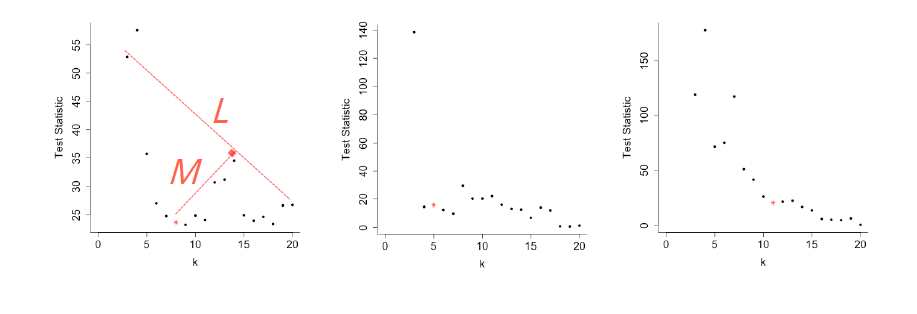
\includegraphics[width=18cm, height=7cm]{t-test}
	\caption{Определения оптимального числа кластеров через t-критерий.}
	\label{t-test}
\end{figure}
	
	
Далее результирующая маска с афтофлуоресцентными объектами получается из маски пересечения, в которой сохранились лишь те регионы идентифицированные как автофлуоресценция.

	
	
	
	
	
\subsection{Расширение автофлуоресцентных областей}
После кластеризации и получения маски автофлуоресцентных объектов применяется функция расширений обастей автофлуоресценции. Наличие этой процедуры объясняется тем что найденные до кластеризации регионы не всегда охватывают нужные области из-за неточных порогов, поэтому нужны удалить дальнейшее "свечение". Суть данного метода состоит в том, чтобы равномерно распределить точки внутри автофлуоресцентного
объекта, а затем расширяться от этих точек во всех направлениях, пока не будет выполнено условие
остановки.

Дадим определение скелету изображения: \textit{Скелет} - множество точек-центров всех вписанных кругов фигуры.

\begin{figure}[H]
	\centering
	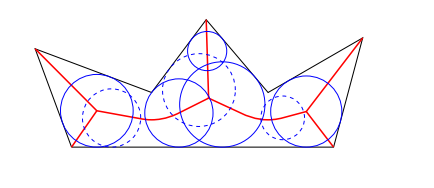
\includegraphics[width=17cm, height=7cm]{skel}
	\caption{Скелет - красная кривая, вписанные круги фигуры - синие.}
	\label{skel}
\end{figure}

Сначала строится скелет маски автофлуоресцентных объектов, далее равномерно распределяются точки по построенному скелету (каждые 20 пикселей). Затем происходит расширение от этих точек до тех пор, пока градиент яркости пикселей от границы области не начнет увеличиваться, указывая на конец или начало соседнего объекта.\cite{Conference}


\begin{figure}[H]
	\centering
	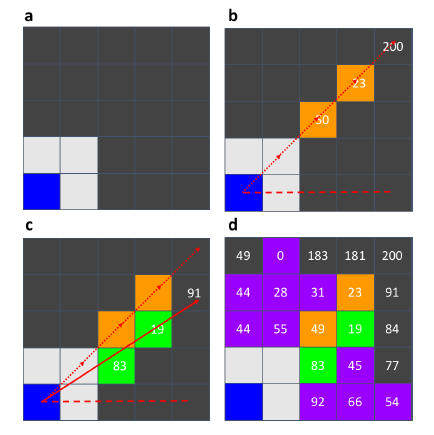
\includegraphics[width=10cm, height=10cm]{expansion}
	\caption{Схема иллюстрирующая шаги алгоритма расширения объектов.}
	\label{expansion}
\end{figure}

На рисунке \ref{expansion} показано, как происходит расширение автофлуоресцентных объектов. Каждый квадрат это пиксель изображения. Белые пиксели - пиксели принадлежащие автофлуоресцентному объекту. Синий пиксель - точка откуда может происходить расширение. Темно-серые пиксели обозначают пиксели, не являющиеся автофлуоресцентным объектом. От точки расширения (синий пиксель) проводится прямая линия. Как только линия достигает края автофлуоресцентного объекта (белые пиксели), она начинает измерять значение пикселей, которые она пересекает. Линия будет продолжать расширяться наружу до тех пор, пока значение
следующего пикселя меньше или равно предыдущему значению пикселя. Все пиксели, удовлетворяющие этому
условию, закрашиваются оранжевым цветом. Новые расширенные пиксели, закрашенные прямой линией исходящей под другим углом, обознаены зеленым и фиолетовыми цветами. Все цветные пиксели теперь образуют новый расширенный объект, который изначально частично состоял из 4
пикселей (левый верхний рисунок а).\cite{Conference}


\subsection{Обзор алгоритма}

У алгоритма AFid существует три вариации:\cite{Conference}


\begin{enumerate}[1.] \label{variations}
	\item Алгоритм считает автофлуоресцентными те области, межканальный коэффициент корреляции Пирсона значений интенсивностей которых больше некоторого изначально заданного значения.
	
	\item Как было указано в \ref{ch2:sec-very-short-title} - вычисляются характеристики для регионов, формируются столбцы со значениями характеристик и далее происхоит кластеризция наборов вычисленных характеристик для каждого региона. Отбирается один кластер у которого среднее значения коэффициента корреляции наибольшее. Все регионы соотвествующие этому кластеру считаются автофлуоресцентными.  В данной вариации алгоритма нужно задать правильное количество кластеров.
	
	\item В последнем варианте алгоритма число кластеров выбирается автоматически. Графически это было показано на рис. \ref{t-test}
\end{enumerate}

Далее представлены псевдокоды алгоритмов обнаружения автофлуоресценции AFid.\cite{Conference}


\begin{algorithm} [H]
	\SetKwFunction{algoDTestsFDSCA}{} 
	\SetKwProg{myalg}{Псевдокод алгоритма автоматического определения оптимального числа кластеров.}{}{} %write in 2nd agrument <<Algorithm>>, <<Procedure>> etc
	\nonl\myalg{\algoDTestsFDSCALING}{ 	
		\KwInput{table - таблица значений характеристик для каждого региона} 	
		\KwOutput{resReg - список регонов соответствующие автофлуоресценции.}
		Stats=[] //список значений статистик для определеня числа кластеров\;
		\For {$(k)\in \overbar{range(2, 20)}$}{
			//кластеризуем наборы характеристик для каждого региона\:
			kmean=KMeans(table)\;
			//находим первые два кластера с макимальным средним значением коорреляций \:
			crMax,crSecMax = findMax(kmean,table)\; 
			//отбираем значения корреляций соответствующие двум кластерам на прошлом шаге\:
			corrVals1,corrVals2 = findCor(crMax,crSecMax)\;
			//находим значение статистики и добавляем в список\:
			Stats.append(ttest(corrVals1, corrVals2))\;	
		}
		kBest = k\_best(Stats) //Определяем оптимальное число кластеров\;
		resRegF=findRegAuto(table) //Находим регионы автофлуоресцении\;
		\Return resReg\;
	}
	\label{alg:AlgoAuto}
\end{algorithm} 


\begin{algorithm}[H]
	\SetKwFunction{algoDTestsFDSCALING}{} 
	\SetKwProg{myalg}{Псевдокод алгоритма детекции автофлуоресценции}{}{} %write in 2nd agrument
	\nonl\myalg{\algoDTestsFDSCALING}{ 	
		\KwInput{ch1 - Первый канал,ch2 - второй канал, resmask - маска пересечения, k - число кластеров, kAuto - если не ноль, то определить оптимальное число кластеров } 	
		\KwOutput{resReg - список регонов соответствующие автофлуоресценции.}
		im1PixStr = regionprops(im1) //поиск регионов в 1 канале\;
		im2PixStr = regionprops(im2) //поиск регионов в 1 канале\;
		minArea = 20\;
		delMin(minArea) //удалить регионы площади меньше minArea\;
		corr=corrcoef(im1Val,im2lVals)//подсчет коэффициентов корреляций \;
		\If{$k > 1$ }{
			std1Vals = std(im1PixStr) //столбец стандартных отклонений\; % or setI() function
			std2Vals = std(im2PixStr)\;
			kurt1Vals = kurt(im1PixStr) //столбец коэффициентов эксцесса\; % or setI() function
			kurt2Vals = kurt(im2PixStr)\; 
			//нормализуем значение полученных столбцов\;
			corrNorm = arctanh(corr) / std(arctanh(corr))\;
			std1ValsNorm = log(std1Vals) / std(arctanh(std1Vals))\;
			std2ValsNorm = log(std2Vals) / std(arctanh(std2Vals))\;
			kurt1ValsNorm = log(kurt1Vals) / std(arctanh(kurt1Vals))\;
			kurt2ValsNorm = log(kurt2Vals) / std(arctanh(kurt2Vals))\;
			//Формируем таблицу столбцов нормированных характеристик для регионов\;
			table=tb(corrNorm,std1ValsNorm...kurt2ValsNorm)\;
			\If{$kAuto > 0$ }{ 
				//Псевдокод алгоритма представлен тут \ref{alg:AlgoAuto}\;
				resRegF=findRegAuto(table) //Находим регионы автофлуоресцении\;
			}
			\uIf{$kAuto = 1$}{
				kmean=KMeans(table)//кластеризуем наборы характеристик\;
				crMax = findMax(kmean,table)//кластер с макимальной коорреляций\; 
				resReg=findReg(crMax)//отбираем соотвествующие регионы \;
			}	
		}
		\Return resReg\;
	}
	\label{alg:AlgoAF}
\end{algorithm} 



\begin{algorithm}[H]
	\SetKwFunction{algoDTestsFDG}{} 
	\SetKwProg{myalg}{Псевдокод алгоритма поиска точек расширения автофлуоресценции}{}{} %write in 2nd agrument
	\nonl\myalg{\algoDTestsFDSCALING}{ 	
		\KwInput{ch1 - Первый канал,ch2 - второй канал, maskAF - маска автофлуоресценции} 	
		\KwOutput{glow1,glow2 - маски точек расширения для 1 и 2 каналов.}
		skel\_af = sk(maskAF)//получаем скелет маски автофлуоресценций\;
		end\_nodes = findEnd(skel\_af)//находим конечные точки скелета, эти точки нужны для определения остальных точек расширения\;
		exp\_points=findExpPoints(skel\_af)//находим остальные точки через каждые trace\_count пикселей, эта константа задается заранее\;
		//удаляем шум путем размытия для нахождения расширений\;
		im1\_blure=GaussianBlur(im1)\;
		im2\_blure=GaussianBlur(im2)\;
		//находим маски расширения для каждого канала используя найденные точки раньше, расширения продолжается до тех пор пока значение интенсивности пикселя не начнет увеличиваться\;
		glow1, glow2 = findExp(im1\_blure, im2\_blure, exp\_points)\;
		\Return glow1, glow2\;
	}
	\label{alg:AlgoEXP}
\end{algorithm} 



На рисунке \ref{af_algo} продемонстрированы шаги алгоритма: сверху(а) показаны шаги для детекции автофлуоресценции, в левом нижнем углу(с) шаги для детекции точек расширения найденных на предыдущем шаге автофлуоресценций. \cite{Conference}

\begin{figure}[H]
	\centering
	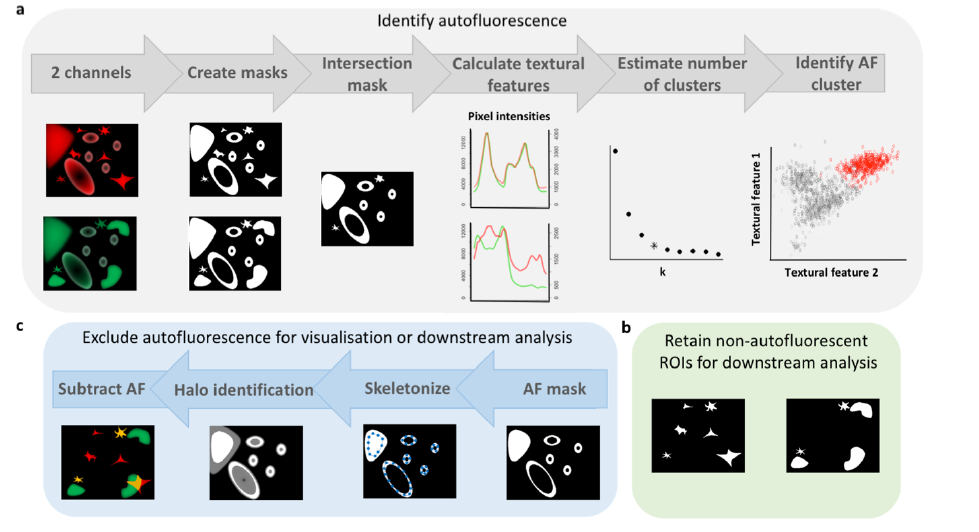
\includegraphics[width=14cm, height=10cm]{af_algo}
	\caption{Иллюстрация шагов алгоритма AFid.}
	\label{af_algo}
\end{figure}
%%% ВНИМАНИЕ: для того, чтобы избежать лишнего отступа между текстом  и формулами, пожалуйста, начинайте формулы без пропуска строки в исходном коде как в строках #2 и #3.
Одиночные формулы также, как и отдельные формулы в составе группы, могут быть размещены в несколько строк. Чтобы выставить номер формулы напротив средней строки, используйте окружение \verb|multlined| из пакета \verb|mathtools| следующим образом \cite{Ganter1999}:
\begin{equation} % \tag{S} % tag - вписывает свой текст 
\label{eq:fConcept-order-G}
\begin{multlined}
(A_1,B_1)\leq (A_2,B_2)\; \Leftrightarrow \\  \Leftrightarrow\; A_1\subseteq A_2\; \Leftrightarrow \\ \Leftrightarrow\; B_2\subseteq B_1. 
\end{multlined}
\end{equation}

	
Используя команду \verb|\labelcref{...}| из пакета \verb|cleveref|, допустимо оформить ссылку на несколько формул, например, (\labelcref{eq:UpArrow-G,eq:DownArrow-G,eq:fConcept-order-G}). % пример оформления одиночной формулы в несколько строк
%
%Пример оформления четырёх иллюстраций в одном текстово-графическом объекте приведён на \firef{fig:spbpu_sc-four-photos}. Это возможно благодаря использованию пакета \verb|subcaption|.

\begin{figure}[ht]
	\adjustbox{minipage=1.3em,valign=t}{\subcaption{}\label{fig:spbpu_sc-a}}%
	\begin{subfigure}[t]{\dimexpr.5\linewidth-1.3em\relax}
		\centering
		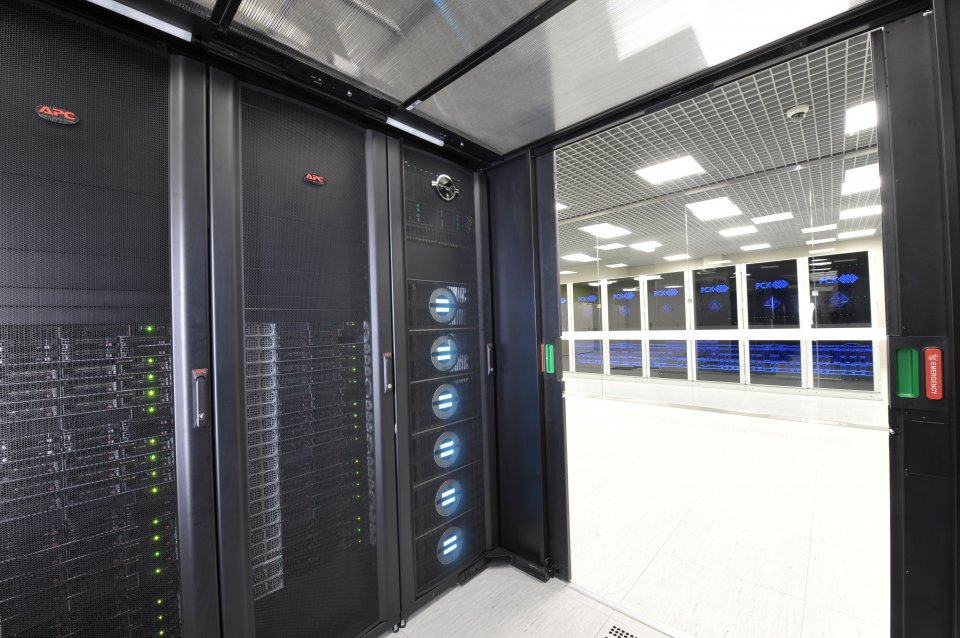
\includegraphics[width=.95\linewidth,valign=t]{my_folder/images/spbpu_sc_system}
	\end{subfigure}
\hfill %выровнять по ширине
	\adjustbox{minipage=1.3em,valign=t}{\subcaption{}\label{fig:spbpu_sc-b}}%
	\begin{subfigure}[t]{\dimexpr.5\linewidth-1.3em\relax}
		\centering
		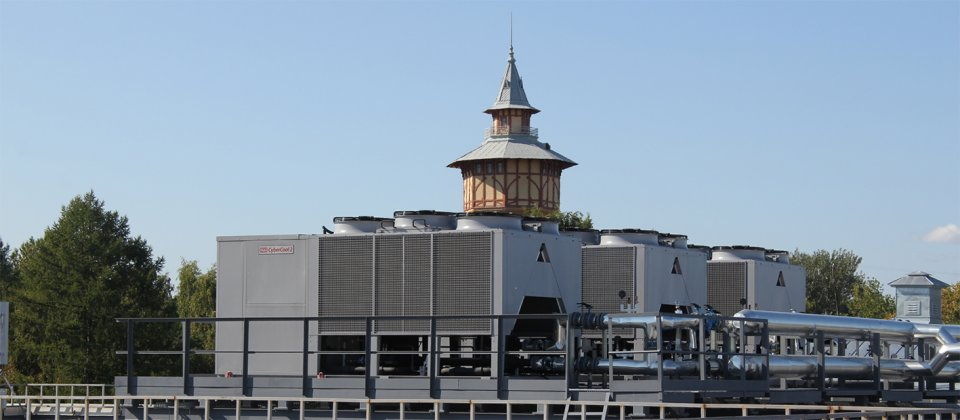
\includegraphics[width=.95\linewidth,valign=t]{my_folder/images/spbpu_sc_refr}
	\end{subfigure}
\\[20pt]
	\adjustbox{minipage=1.3em,valign=t}{\subcaption{}\label{fig:spbpu_sc-c}}%
\begin{subfigure}[t]{\dimexpr.5\linewidth-1.3em\relax}
	\centering
	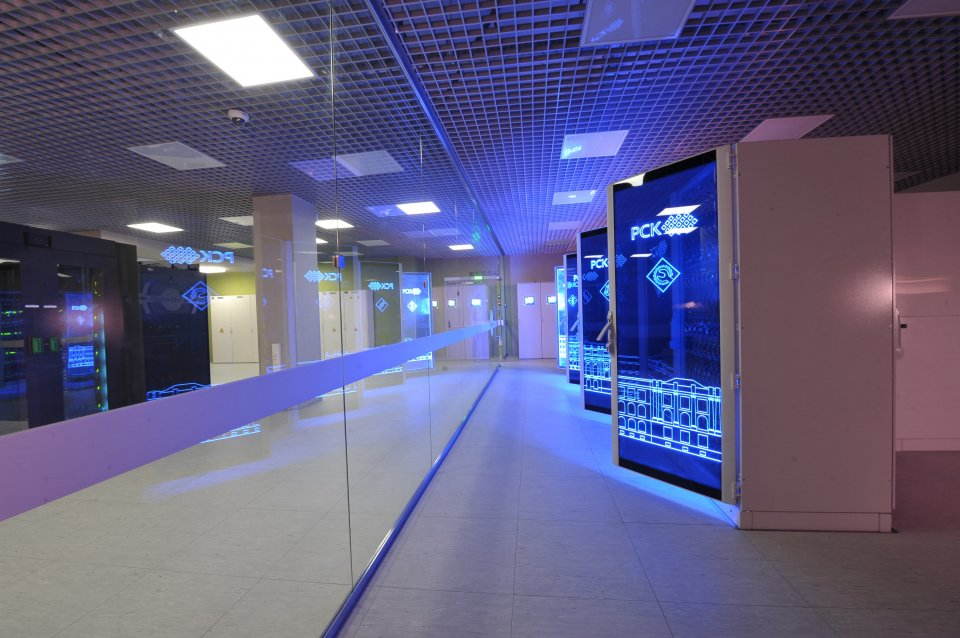
\includegraphics[width=.95\linewidth,valign=t]{my_folder/images/spbpu_sc_hall}
\end{subfigure}%
\hfill %выровнять по ширине
\adjustbox{minipage=1.3em,valign=t}{\subcaption{}\label{fig:spbpu_sc-d}}%
\begin{subfigure}[t]{\dimexpr.5\linewidth-1.3em\relax}
	\centering
	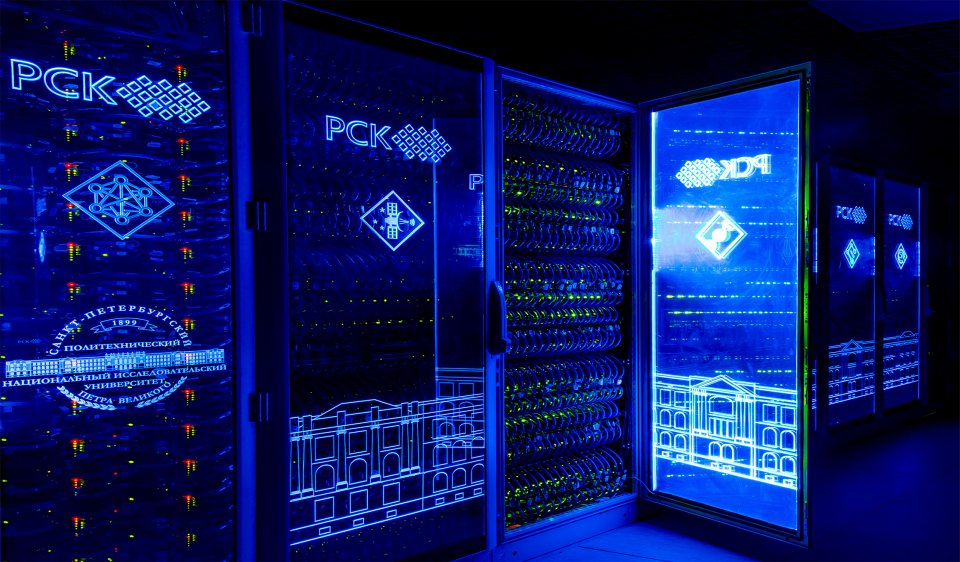
\includegraphics[width=.95\linewidth,valign=t]{my_folder/images/spbpu_sc_box}
\end{subfigure}
\captionsetup{justification=centering} %центрировать
\caption{Фотографии суперкомпьютерного центра СПбПУ \cite{spbpu-gallery}: {\itshape a} --- система хранения данных и узлы NUMA-вычислителя; {\itshape b} --- холодильные машины на крыше научно-исследовательского корпуса; {\itshape c} --- машинный зал; {\itshape d} --- элементы вычислительных устройств} 
\label{fig:spbpu_sc-four-photos}
\end{figure}

Далее можно ссылаться на составные части данного рисунка как на самостоятельные объекты: \firef{fig:spbpu_sc-a}, \firef{fig:spbpu_sc-b}, \firef{fig:spbpu_sc-c}, \firef{fig:spbpu_sc-d} или на три из четырёх изображений одновременно: рис.\labelcref{fig:spbpu_sc-a,fig:spbpu_sc-b,fig:spbpu_sc-c}. % пример подключения 4х иллюстраций в одном рисунке
%
%%На \firef{fig:spbpu_whitehall-three-photos} приведены три картинки под~общим номером и~названием, но с раздельной нумерацией подрисунков посредством пакета \verb|subcaption|.
%
\begin{figure}[!htbp]
	\adjustbox{minipage=1.3em,valign=t}{\subcaption{}\label{fig:spbpu_whitehall-a}}%
	\begin{subfigure}[t]{\dimexpr.3\linewidth-1.3em\relax}
		\centering
		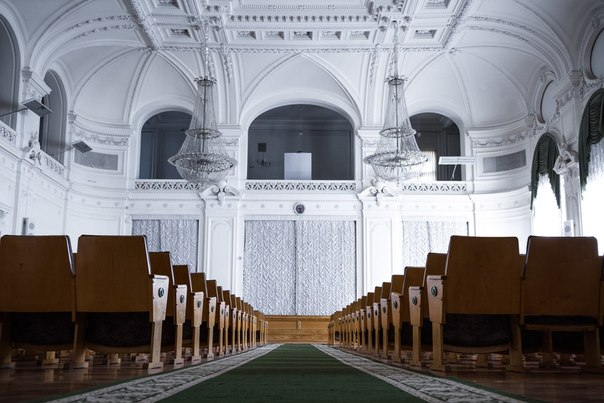
\includegraphics[width=.95\linewidth,valign=t]{my_folder/images//spbpu_whitehall}
	\end{subfigure}
	\hfill %выровнять
	\adjustbox{minipage=1.3em,valign=t}{\subcaption{}\label{fig:spbpu_whitehall-b}}%
	\begin{subfigure}[t]{\dimexpr.3\linewidth-1.3em\relax}
		\centering
		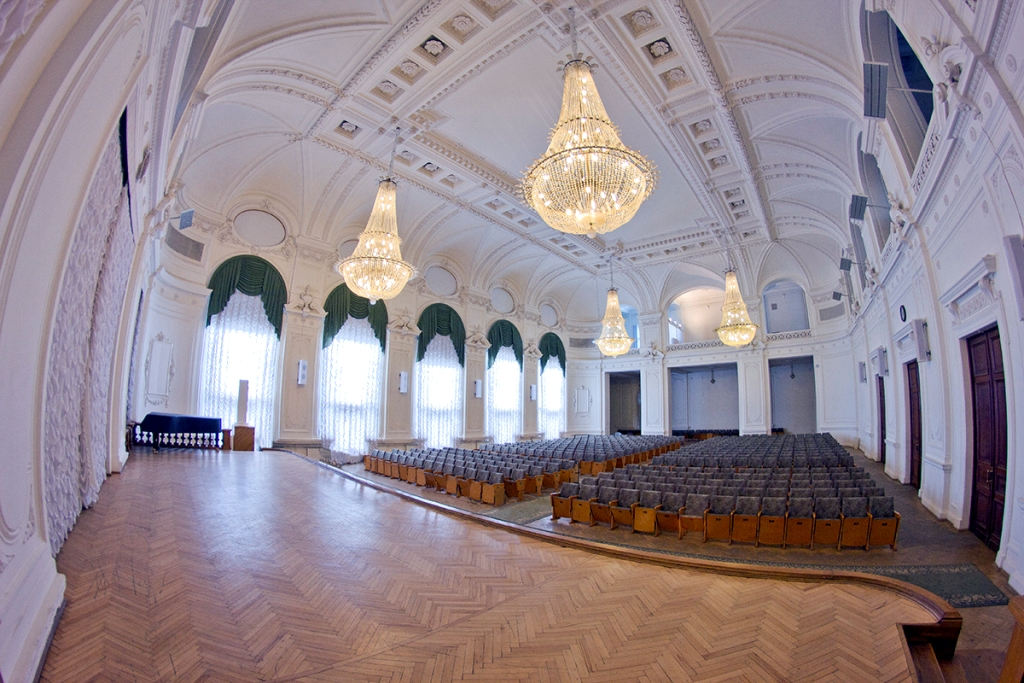
\includegraphics[width=.95\linewidth,valign=t]{my_folder/images//spbpu_whitehall_ligh}
	\end{subfigure}
	\hfill %выровнять
		\adjustbox{minipage=1.3em,valign=t}{\subcaption{}\label{fig:spbpu_whitehall-c}}%
	\begin{subfigure}[t]{\dimexpr.3\linewidth-1.3em\relax}
		\centering
		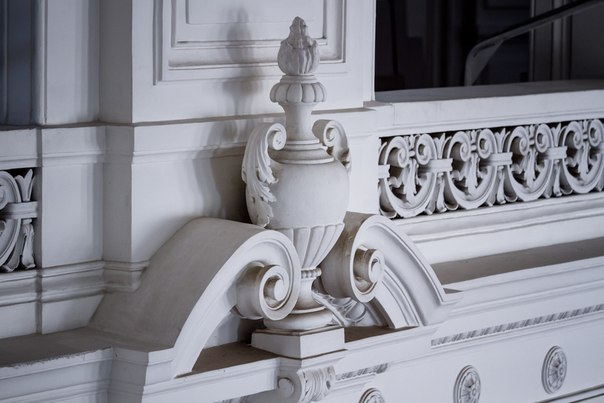
\includegraphics[width=.95\linewidth,valign=t]{my_folder/images//spbpu_whitehall_sculpture}
	\end{subfigure}%
\captionsetup{justification=centering} %центрировать
	\caption{Фотографии Белого зала СПбПУ \cite{spbpu-gallery}, в том числе: {\itshape a} --- со стороны зрителей; {\itshape b} --- со стороны сцены; {\itshape c} --- барельеф}\label{fig:spbpu_whitehall-three-photos}  
\end{figure}

Далее можно ссылаться на три отдельных рисунка: \firef{fig:spbpu_whitehall-a}, \firef{fig:spbpu_whitehall-b} и \firef{fig:spbpu_whitehall-c}. % пример подключения 3х иллюстрации в одном рисунке
%%
%%На \firef{fig:spbpu_main_bld-two-photos} приведены две картинки под~общим номером и~названием.


\begin{figure}[!htbp]
	\adjustbox{minipage=1.3em,valign=t}{\subcaption{}\label{fig:spbpu_main_bld_entrance_autumn}}%
	\begin{subfigure}[t]{\dimexpr.5\linewidth-1.3em\relax} %разрешили выделить 0,5 стр в ширину на рисунок
		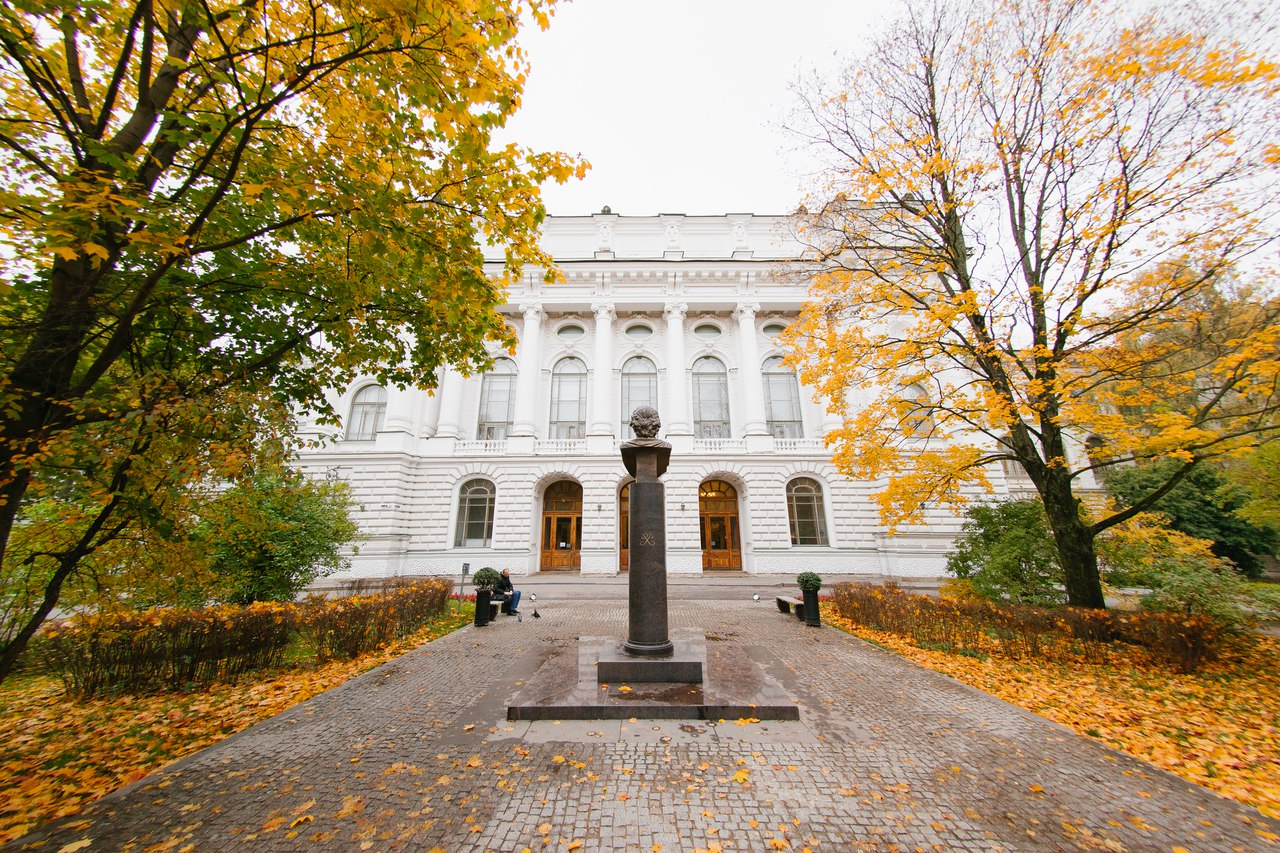
\includegraphics[height=0.20\textheight,valign=t]{my_folder/images//spbpu_main_bld_entrance_autumn} %высоту рисунка выставили как 0,3 от высоты наборного поля
	\end{subfigure}
%	\hfill %выровнять по ширине
	\adjustbox{minipage=1.3em,valign=t}{\subcaption{}\label{fig:spbpu_main_bld_whitehall}}%
	\begin{subfigure}[t]{\dimexpr.5\linewidth-1.3em\relax}%разрешили выделить 0,5 стр в ширину на рисунок
		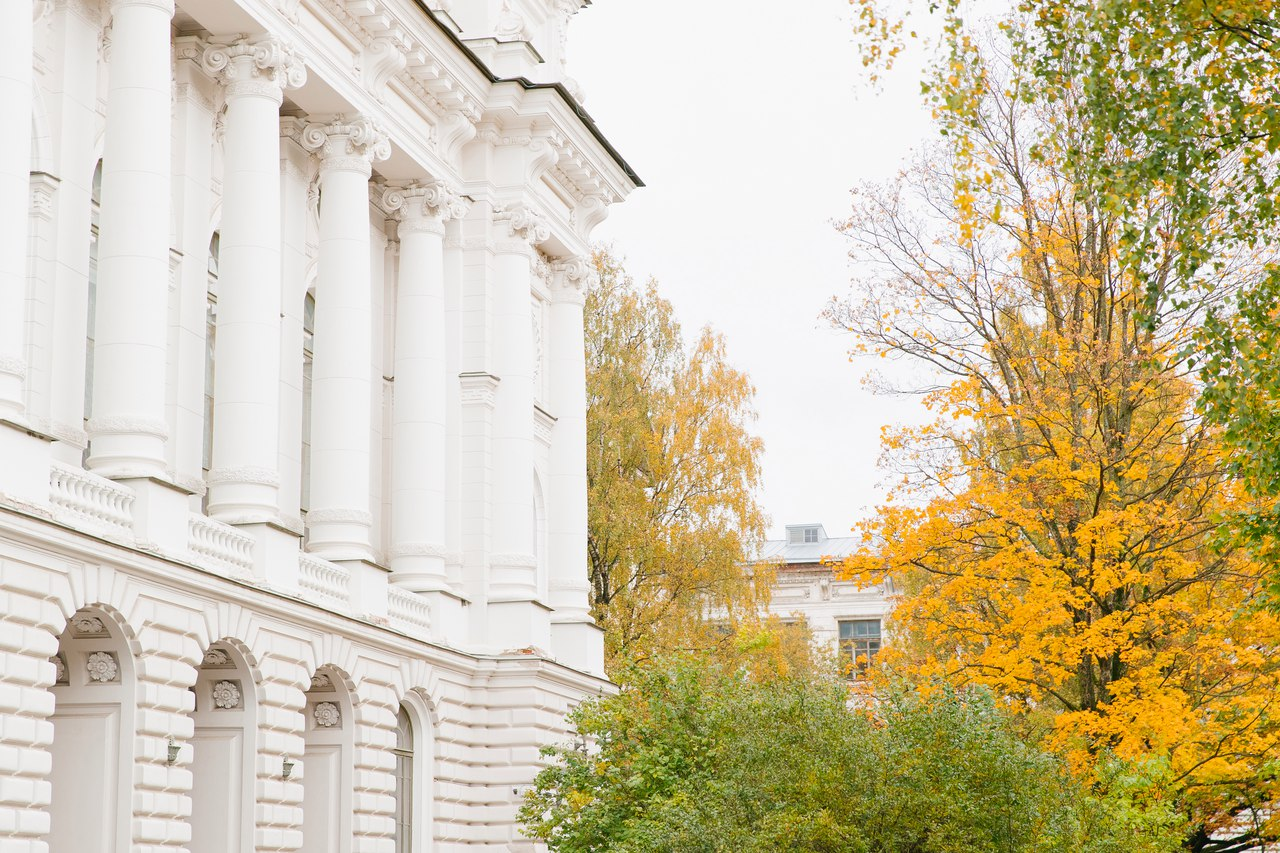
\includegraphics[height=0.20\textheight,valign=t]{my_folder/images//spbpu_main_bld_whitehall}%высоту рисунка выставили как 0,3 от высоты наборного поля
	\end{subfigure}
\captionsetup{justification=centering} %центрировать
	\caption{Вид на главное здание СПбПУ \cite{spbpu-gallery}, включая: {\itshape a} --- вход со стороны парка осенью; {\itshape b}~--- окна Белого зала}\label{fig:spbpu_main_bld-two-photos} 
\end{figure}

На \firef{fig:spbpu_main_bld_entrance_autumn} изображен вход со стороны парка СПбПУ осенью, а на \firef{fig:spbpu_main_bld_whitehall}~--- окна Белого зала. % пример подключения 2х иллюстраций в одном рисунке
%
%Приведём пример табличного представления данных с записью продолжения на следующей странице на \taref{tab:long}.

%%% отладка longtable
%% 1) для контроля выхода таблицы за границы полей выставляем showframe в \geometry{}, см настройки
%% 2) используем \\* для запрета переноса определенной строки или средства из:
%% https://tex.stackexchange.com/q/344270/44348
%% 3) в крайнем случае для принудительного переноса таблицы на новую страницу используем \pagebreak после \\
\noindent % for correct centering
\begingroup
\centering
\small %выставляем шрифт в 12bp
\begin{longtable}[c]{|l|l|l|l|l|l|}
	\caption{Пример задания данных из \cite{Peskov2004} (с повтором для переноса таблицы на новую страницу)}%
	\label{tab:long}% label всегда желательно идти после caption
	\\
	\hline
	$G$&$m_1$&$m_2$&$m_3$&$m_4$&$K$\\ \hline
	1&2&3&4&5&6\\ \hline
	\endfirsthead%
	\captionsetup{format=tablenocaption,labelformat=continued} % до caption!
	\caption[]{}\\ % печать слов о продолжении таблицы
	\hline
	1&2&3&4&5&6\\ \hline
	\endhead
	\hline
	\endfoot
	\hline
	\endlastfoot
	$g_1$&0&1&1&0&1\\ \hline
	$g_2$&1&2&0&1&1\\ \hline
	$g_3$&0&1&0&1&1\\ \hline
	$g_4$&1&2&1&0&2\\ \hline
	$g_5$&1&1&0&1&2\\ \hline
	$g_6$&1&1&1&2&2\\ \hline
%
	$g_1$&0&1&1&0&1\\ \hline 
	$g_2$&1&2&0&1&1\\ \hline
	$g_3$&0&1&0&1&1\\ \hline
	$g_4$&1&2&1&0&2\\ \hline \noalign{\penalty-5000} % способствуем переносу на следующую стр
	$g_5$&1&1&0&1&2\\ \hline 
	$g_6$&1&1&1&2&2\\ \hline
%
	$g_1$&0&1&1&0&1\\ \hline 
	$g_2$&1&2&0&1&1\\ \hline
	$g_3$&0&1&0&1&1\\ \hline
	$g_4$&1&2&1&0&2\\ \hline
	$g_5$&1&1&0&1&2\\ \hline
	$g_6$&1&1&1&2&2\\ \hline
%		
	$g_1$&0&1&1&0&1\\ \hline 
	$g_2$&1&2&0&1&1\\ \hline
	$g_3$&0&1&0&1&1\\ \hline
	$g_4$&1&2&1&0&2\\ \hline
	$g_5$&1&1&0&1&2\\ \hline
	$g_6$&1&1&1&2&2\\ \hline
%
	$g_1$&0&1&1&0&1\\ \hline 
	$g_2$&1&2&0&1&1\\ \hline
	$g_3$&0&1&0&1&1\\ \hline
	$g_4$&1&2&1&0&2\\ \hline
	$g_5$&1&1&0&1&2\\ \hline
	$g_6$&1&1&1&2&2\\ \hline
%
	$g_1$&0&1&1&0&1\\ \hline 
	$g_2$&1&2&0&1&1\\ \hline
	$g_3$&0&1&0&1&1\\ \hline
	$g_4$&1&2&1&0&2\\ \hline
	$g_5$&1&1&0&1&2\\ \hline
	$g_6$&1&1&1&2&2\\ \hline
%
	$g_1$&0&1&1&0&1\\ \hline 
	$g_2$&1&2&0&1&1\\ \hline
	$g_3$&0&1&0&1&1\\ \hline
	$g_4$&1&2&1&0&2\\ \hline
	$g_5$&1&1&0&1&2\\ \hline
	$g_6$&1&1&1&2&2\\ \hline
\end{longtable}
\normalsize% возвращаем шрифт к нормальному
\endgroup % пример подключения таблицы на несколько страциц
%
%
%\begin{table} [htbp]% Пример оформления таблицы
%	\centering\small
%	\caption{Пример представления данных для сквозного примера по ВКР \cite{Peskov2004}}%
%	\label{tab:ToyCompare}		
%		\begin{tabular}{|l|l|l|l|l|l|}
%			\hline
%			$G$&$m_1$&$m_2$&$m_3$&$m_4$&$K$\\
%			\hline
%			$g_1$&0&1&1&0&1\\ \hline
%			$g_2$&1&2&0&1&1\\ \hline
%			$g_3$&0&1&0&1&1\\ \hline
%			$g_4$&1&2&1&0&2\\ \hline
%			$g_5$&1&1&0&1&2\\ \hline
%			$g_6$&1&1&1&2&2\\ \hline		
%		\end{tabular}
%%	\caption*{\raggedright\hspace*{2.5em} Составлено (или/и рассчитано) по \cite{Peskov2004}} %Если проведена авторская обработка или расчеты по какому-либо источнику	
%	\normalsize% возвращаем шрифт к нормальному
%\end{table}
%
%
%
%%% please, before using, read the author guide carefully
%
%\noindent % for correct centering
\begin{minipage}{\textwidth}
	\vspace{\mfloatsep} % интервал 
	\centering\small
	\captionof{table}{Пример задания данных в табличном виде из \cite{Peskov2004} (с помощью окружения minipage)}%
	\label{tab:ToyCompare-Peskov-minipage}
	\begin{tabular}{|l|l|l|l|l|l|}
	\hline
	$G$&$m_1$&$m_2$&$m_3$&$m_4$&$K$\\
	\hline
	$g_1$&0&1&1&0&1\\ \hline
	$g_2$&1&2&0&1&1\\ \hline
	$g_3$&0&1&0&1&1\\ \hline
	$g_4$&1&2&1&0&2\\ \hline
	$g_5$&1&1&0&1&2\\ \hline
	$g_6$&1&1&1&2&2\\ \hline
	\hline		
	\end{tabular}
\vspace{\mfloatsep} % интервал 
\normalsize %восстанавливаем шрифт 	
\end{minipage} % пример подключения minipage
%
%\noindent % for correct centering
\begin{minipage}{\textwidth}
	\centering
	\vspace{\mfloatsep} % интервал  	
	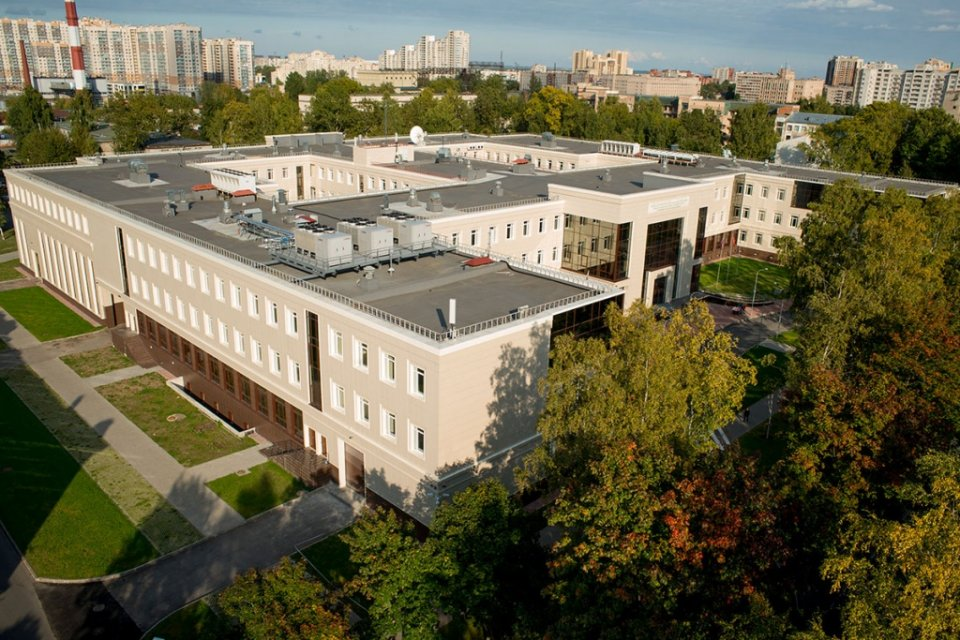
\includegraphics[keepaspectratio=true,scale=0.27] {my_folder/images/spbpu_new_bld_autumn}
	\captionof{figure}{Новый научно-исследовательский корпус СПбПУ \cite{spbpu-gallery} (с помощью окружения minipage)}\label{fig:spbpu-new-bld-autumn-minipage}  
	\vspace{\mfloatsep} % интервал  	
\end{minipage} % пример подключения minipage
%
%
%
%
%Вопросы форматирования текстово-графических объектов (окружений) не регламентированы в известных нам ГОСТах, поэтому предлагаем придерживаться следующих правил:

\begin{itemize}
	\item \textbf{полужирный текст} рекомендуем использовать только для названий стандартных окружений с нумерационной частью, например, для представления \textit{впервые}: \textbf{определение 1.1}, \textbf{теорема 2.2}, \textbf{пример 2.3}, \textbf{лемма 4.5};
	
	\item \textit{курсив} рекомендуем использовать только для выделения переменных в формулах, служебной информации об авторах главы (статьи), важных терминов, представляемых по тексту, а также для всего тела окружений, связанных с получением \textit{новых существенных результатов и их доказательством}: теорема, лемма, следствие, утверждение и другие.
\end{itemize}

 
%
%По аналогии с нумерацией формул, рисунков и таблиц нумеруются и иные текстово-графические объекты, то есть включаем в нумерацию номер главы, например: теорема 3.1. для первой теоремы третьей главы монографии. Команды \LaTeX{} выставляют нумерацию и форматирование автоматически. Полный перечень команд для подготовки текстово-графических и иных объектов находится в подробных методических рекомендациях \cite{spbpu-bci-template-author-guide}. 
%
%
%Для удобства авторов названия стандартных окружений, рекомендованных к использованию, приведены в \taref{tab:enum-std}, а в \taref{tab:enum-spbpu}  перечислены имена специально разработанных окружений для шаблонов SPbPU.

% и примеры их оформления на псевдокоде (см. \cite{cite-spbpu-bci}).


%https://tex.stackexchange.com/questions/2651/should-i-use-center-or-centering-for-figures-and-tables


	\begin{table} [htbp]% Пример записи таблицы с номером, но без отображаемого наименования
	\centering\small
	\caption{Стандартные окружения}%
	\label{tab:enum-std}
	 \begin{Spacing}{\Single} % Одинарный интервал между строками текста 
	  \renewcommand*{\arraystretch}{1.5} % Полуторный интервал между ячейками таблицы
		\begin{tabular}{|l|p{11cm}|} 
			\hline
			Название окружения&Назначение\\
			\hline
			\verb|center| &	центрирование, аналог команды \verb|\centering|, но с добавлением нежелательного пробела, поэтому лучше избегать применения \verb|center|\\ \hline
			\verb|itemize| &{перечисления, в которых нет необходимости нумеровать  пункты (немаркированные списки)} \\ \hline
			\verb|enumerate| & перечисления с нумерацией (немаркированные списки) \\ \hline
			\verb|refsection| & создание отдельных библиографических списков для глав \\ \hline
			\verb|tabular| & оформление таблиц \\ \hline
			\verb|table|   &{автоматическое перемещение по тексту таблиц, оформленных, например, с помощью \verb|tabular|, для минимизации пустых пространств} \\ \hline
			\verb|longtable| & оформление многостраничных таблиц \\ \hline
			\verb|tikzpicture| & создание иллюстраций с помощью пакета \verb|tikz| \cite{ctan-tikz} \\ \hline
			\verb|figure| &{автоматическое перемещение по тексту рисунков, оформленных например, с помощью \verb|tikz| или подключенных с помощью команды \verb|\includegraphics|, для минимизации пустых пространств} \\ \hline 
			\verb|subfigure| & оформление вложенных рисунков в составе \verb|figure| \\ \hline
			\verb|algorithm| &{оформление псевдокода на основе пакета \verb|algorithm2e| \cite{ctan-algorithm2e}} \\ \hline
			\verb|minipage| & {оформление рисунков и таблиц без функций автоматического перемещения по тексту для  минимизации пустых пространств} \\ \hline
			\verb|equation| & {оформление выключенных (не встроенных в текст с помощью \verb|$...$|) одиночных формул на одной строке} \\ \hline
			\verb|multilined| &{оформление выключенных (не встроенных в текст с помощью \verb|$...$|) одиночных формул в несколько строк} \\ \hline 
			\verb|aligned| &{оформление нескольких формул с выравниванием по символу \verb|&|.} \\ \hline
	\end{tabular}
	\end{Spacing}
%	\normalsize
	\end{table}

На базе пакета \verb|tikz| разработано большое количество расширений \cite{ctan-tikz}, например, \verb|tikzcd|, которые мы рекомендуем использовать для оформления иллюстраций.

	\begin{table} [htbp]% Пример записи таблицы с номером, но без отображаемого наименования
	\centering\small
	\caption{Специальные окружения}%
	\label{tab:enum-spbpu}
		\begin{tabular}{|l|l|}
			\hline
			Название окружения & Текстово-графический объект\\
			\hline
			\verb|abstr|	 & реферат (abstract) \\ \hline
			\verb|m-theorem| & теорема \\ \hline 
			\verb|m-corollary| & следствие \\ \hline
			\verb|m-proposition| & утверждение \\ \hline
			\verb|m-lemma|   & лемма \\ \hline
			\verb|m-axiom| & аксиома \\ \hline
			\verb|m-example| & пример \\ \hline
			\verb|m-definition| &  определение \\ \hline
			\verb|m-condition| & условие \\ \hline
			\verb|m-problem| & проблема \\ \hline
			\verb|m-exercise| & упраженение \\ \hline
			\verb|m-question| & вопрос \\ \hline
			\verb|m-hypothesis| & гипотеза \\ \hline
		\end{tabular}	
	\normalsize
\end{table}

В случае, если авторам потребовалось новое окружение, то создать его можно в файле в файле \texttt{my\_fol\-der/{}my\_set\-tings.tex} согласно правилам, приведённым ниже.

\begin{enumerate}[1.]
	\item Для перехода в режим создания окружений следует указать:
	\begin{itemize}
		\item \verb|\theoremstyle{myplain}| --- окружения с доказательствами или аксиомами
		\item \verb|\theoremstyle{mydefinition}| --- окружения, не связанные с доказательствами или аксиомами.
	\end{itemize}
	\item В команде создания окружения следует ввести краткий псевдоним (\verb|m-new-env|) и отображаемое в pdf имя окружения (\verb|Название_окружения|):
	\begin{itemize}
		\item \texttt{\textbackslash{}newtheorem\{m-new-env-second\}\{Название\_окруже\-ния\}\-[chap\-ter]}.
	\end{itemize}
\end{enumerate}


%\begin{m-new-env-first}
%	Тест первого пользовательского окружения
%\end{m-new-env-first}
%
%\begin{m-new-env-second}
%	Тест второго пользовательского окружения
%\end{m-new-env-second} % список некоторых окружений
%
%
%\begin{m-theorem}[о чем-то конкретном] %при необходимости в [] можно записать название теоремы или убрать его
	\label{th:ex} 
	% \index только для принятых работ
	% шаблон записи теоремы в Предметный указатель
	\index[ru]{теорема!название\_теоремы или о чём} %ключевое слово <<теорема>> не менять
	\index[en]{theorem!1-3 words for detail or description}
	% пример записи алгоритма в Предметный указатель
	\index[ru]{теорема!о неполноте}
	\index[en]{theorem!about incompleteness}
	% пример записи алгоритма в Предметный указатель
	\index[ru]{теорема!о жизни}
	\index[en]{theorem!about life}
	Текст теоремы полностью выделен курсивом. Допустимо математические символы не выделять курсивом, если это искажает их значения. Используется абзацный отсуп, так как ``Абзацы в тексте начинают отступом'' в соответствии с ГОСТ 2.105--95. Название теоремы допустимо убрать. Доказательство окончено.
\end{m-theorem}
Доказательство теоремы \ref{th:ex}, леммы, утверждений, следствий и других подобных окружений (в последнем абзаце) завершаем предложением в котором сказано, что доказательство окончено. Например, доказательство теоремы \ref{th:ex} окончено.

Тело доказательства не выделяется курсивом.
Тело следующих окружений также не выделяется сплошным курсивом: определение, условие, проблема, пример, упражнение, вопрос, гипотеза и другие. %пример оформления теоремы
%
%
%\begin{m-definition}[термин] %при необходимости в [] можно записать название определения или убрать его
	\label{def:ex}
	% \index только для принятых работ
	% шаблон записи определения в Предметный указатель 
	\index[ru]{название\_определения!1-3 уточняющих слова или~ничего}
	\index[en]{definition\_title!1-3 words for detail or~without "!-part}
	% пример записи определения в Предметный указатель 
	\index[ru]{и-тест!хороший!наилучший}
	\index[en]{i-test!good!best}
	% пример записи определения в Предметный указатель 
	\index[ru]{и-тест!замкнутый}
	\index[en]{i-test!closed}
	В тексте определения только {\itshape важные термины} выделяются курсивом. Если определение носит лишь вспомогательный характер, то допустимо не использовать окружение \texttt{m-definition}, представляя текст определения в обычном абзаце. Ключевые термины при этом обязательно выделяются курсивом.
\end{m-definition} %пример оформления определения
%
%
%Вместо теоремо-подобных окружений для вставки небольших текстово-графических объектов иногда используются команды. Типичным примером такого подхода является команда \verb|\footnote{text}|\footnote{Внимание! Команда вставляется непосредственно после слова, куда вставляется сноска (без пробела). Лишние пробелы также не указываются внутри команды перед и после фигурных скобок.}, где в аргументе \verb|text| указывают текст \textit{подстрочной ссылки (сноски)}.В них \textit{нельзя добавлять веб-ссылки или цитировать литературу}. Для этих целей используется список литературы. Нумерация сносок сквозная по ВКР без точки на конце выставляется в шаблоне автоматически, однако в каждом приложении к ВКР нумерация, зависящая от номера приложения, выставляется префикс <<П>>, например <<П1.1>> --- первая сноска первого приложения. 




%\FloatBarrier % заставить рисунки и другие подвижные (float) элементы остановиться


%\section{Выводы} \label{ch2:conclusion}
%
%Текст заключения ко второй главе. Пример ссылок \cite{Article,Book,Booklet,Conference,Inbook,Incollection,Manual,Mastersthesis,Misc,Phdthesis,Proceedings,Techreport,Unpublished,badiou:briefings}, а также ссылок с указанием страниц, на котором отображены те или иные текстово-графические объекты  \cite[с.~96]{Naidenova2017} или в виде мультицитаты на несколько источников \cites[с.~96]{Naidenova2017}[с.~46]{Ganter1999}. Часть библиографических записей носит иллюстративный характер и не имеет отношения к реальной литературе. 
%
%Короткое имя каждого библиографического источника содержится в специальном файле \verb|my_biblio.bib|, расположенном в папке \verb|my_folder|. Там же находятся исходные данные, которые с помощью программы \texttt{Biber} и стилевого файла \texttt{Biblatex-GOST} \cite{ctan-biblatex-gost} приведены в списке использованных источников согласно ГОСТ 7.0.5-2008.
%Многообразные реальные примеры исходных библиографических данных можно посмотреть по ссылке \cite{ctan-biblatex-gost-examples}.
%
%Как правило, ВКР должна состоять из четырех глав. Оставшиеся главы можно создать по образцу первых двух и подключить с помощью команды \verb|\input| к исходному коду ВКР. Далее в приложении \ref{appendix-MikTeX-TexStudio} приведены краткие инструкции запуска исходного кода ВКР \cite{latex-miktex,latex-texstudio}.
%
%В приложении \ref{appendix-extra-examples} приведено подключение некоторых текстово-графических объектов. Они оформляются по приведенным ранее правилам. В качестве номера структурного элемента вместо номера главы используется <<П>> с номером главы. Текстово-графические объекты из приложений не учитываются в реферате.



%% Вспомогательные команды - Additional commands
%
%\newpage % принудительное начало с новой страницы, использовать только в конце раздела
%\clearpage % осуществляется пакетом <<placeins>> в пределах секций
%\newpage\leavevmode\thispagestyle{empty}\newpage % 100 % начало новой страницы